\documentclass{article}

\usepackage[utf8]{inputenc}
\usepackage{graphicx}
\usepackage{citesort}
\usepackage{multirow}
\usepackage{rotating}
\usepackage[all]{xy}
\usepackage{amsmath}
\usepackage{amssymb}

\begin{document}

\title{
  Whitepaper:  The Universal Recommender \\
  \large{A Recommender System for Complex Semantic Networks}
}
\author{
  Jérôme Kunegis, Alan Said and Winfried Umbrath \\
  \small{Technische Universität, DAI-Labor, Germany} \\
  \texttt{\{kunegis,alan.said,winfried.umbrath\}@dai-lab.de} \\
}

\date{September 2009}

\maketitle

\begin{abstract}
We describe the Universal Recommender, a semantic recommendation engine
that applies to semantic datasets, being
independent of a specific data model.  
The Universal Recommender generalizes domain-specific recommenders such
as content-based, collaborative, social, bibliographic, lexicographic and
hybrid recommenders. 
To achieve good recommendation accuracy, several novel machine learning
and optimization problems are solved by the Universal Recommender.   
\end{abstract}

\section{Introduction}
In the field of information retrieval, a recommender system is any
system that is able to find entities in a dataset that may be of
interest to the user.  In contrast to search engines, recommender systems
do not base their results on a \emph{query}, instead relying on user
profiles. 

In the general case, a recommender system applies to a dataset 
described by a data model containing entities (such as users and
items) and relationships (such as ratings and social links).  
In the simplest recommender system, the data consists of one
relationship type connecting one or two entity types.  In more complex
cases, the dataset contains multiple relationship types connecting any
number of entity types.

The simple case of only one relationship type corresponds to several
well-studied recommendation subproblems, such as link prediction,
collaborative filtering, citation analysis, etc.  In the case of
multiple relationship types, hybrid recommenders are normally used.
Hybrid recommenders are typically described as combining several simple 
recommenders, each corresponding to one relationship type.  This
approach however has two problems:  First, by considering only subsets
of the dataset, latent relations between entities from different
relationship types may be missed.
Second, for each dataset, a new hybrid recommender has to be developed.  

To avoid these problems we propose the Universal Recommender, a
recommendation engine with the following features.
\begin{itemize}
\item It applies to datasets with any number of entity and relationship
  types. 
\item It learns all its parameters without human intervention.
\end{itemize}
The first requirement ensures the recommender can be applied to future
datasets whose structure is as-yet unknown.  The second requirement is
more critical:  Since a recommender using complex datasets has a large
set of parameters, a complex recommender runs the risk of either
overfitting the data or having very low recommendation quality. 
The main challenges of the Universal Recommender are therefore a series
of machine learning problems related to the complexity of semantic
networks. 

We begin the paper by reviewing typical recommendation datasets and
tasks, and give known solutions to specific recommendation problems.
We then describe the unified data model and the general approach of the
Universal Recommder, and introduce the machine learning and optimization
problems that it will have to solve.  We finish by describing the case
study of an IPTV recommender system.  

\section{Complex Semantic Networks}
In this section, we give examples of classical recommendation scenarios
motivating the comlpexity of typical recommendation datasets. We also
review existing solutions for partial recommendation problems.  

We describe all cases in the context of the Internet Protocol Television
recommender system~\cite{b430}.  In the IPTV recommendation setting we want
to recommend a TV program to a user.  In the following examples we
describe classical recommendation settings applied to our scenario.  

\subsection{Content-based Filtering}
An early form of recommendation consists in content-based filtering.  As
in search engines, content-based filtering considers the content of
items.  While search engines require the user to enter a specific
keyword for searching, content-based recommenders usually take keyword
from another source, for instance a profile filled out by the user
(containing words describing his interests), or from documents already
seen or rated.

The following diagram shows a situation in which a user-item
recommendation is found by analysis common features of two items. 
Arrows represent known relationships and the dotted arrow represents the
relationship to predict.  $U$, $I$ and $W$ represent users, items and
words respectively. 

\begin{displaymath}
  \xymatrix{ 
    U_1 \ar@{.>}[r] \ar[rd] & I_1 \ar[r] \ar[rd] & W_1 \\
    & I_2 \ar[ru] \ar[r]  & W_2
  }
\end{displaymath}


For our IPTV system, each TV program would have a description of
its content.  The weight of single keywords for each TV program is
then computed by the tf-idf measure.  
This example already shows a limitation of the content-based approach:
Because the TV program descriptions are much shorter than typical
documents, the tf-idf measure will be less accurate. 

\subsection{Collaborative Filtering}
While the content-based approach is simple (being essentially a search
engine), it requires the user to enter a profile.  If our IPTV
tracks the programs watched by each user, this information can be
exploited directly giving collaborative filters.   

\begin{displaymath}
  \xymatrix{
    U_1 \ar@{.>}[r] \ar[rd] & I_1 \\
    U_2 \ar[ru] \ar[r] & I_2 
  }
\end{displaymath}

The general idea is the following:  If we known which TV programs the user
has seen, then we can use this information directly, without needing content
information.  To do this, a collaborative recommender system must
consider the behavior of other users:  If another user has seen the same
TV program as a given user, we can recommend other TV programs seen by that
other user.  The result is a recommendation system that does not need
any content information.  Therefore, collaborative recommenders are
often used in scenarios where no or little content is available:  for
instance movies or jokes~\cite{b7}.  For our IPTV recommender,
this means we don't have to rely on content descriptions, and we may
recommend TV programs that don't have a description. 

What is more, a collaborative recommender can make use of explicit 
\emph{ratings}.  Compared to the typical ``has-seen'' information,
ratings have the advantage of also admitting negative values, modeling
dislike.  To collect such ratings, we either ask users to explicitly
rate TV programs, or derive ratings from user behavior.  If for instance
a user stops a TV program after just a few minutes, we may assign to it
a negative rating. 

\subsection{Social Networks and Link Prediction}
A further type of recommender is given when links are known between
users.  For instance, if IPTV users can maintain a buddy list, 
we may recommend the favorite items of a given user's buddies.  
This type of recommendation is particularly useful when trust is
important.  In this case, a trust measure can be defined between users,
denoting the level of confidence a user has in another user's tastes.  

\begin{displaymath}
  \xymatrix{
    U_1 \ar@{.>}[r]  \ar[d] & I_1 \\
    U_2 \ar[ur]
  }
\end{displaymath}

In a addition to friendship and trust, which are positive relationships,
we may allow users to mark other users as enemies, representing
distrust~\cite{b325,kunegis:slashdot-zoo}.   

% missing subsection:  citations/hyperlinks.  Does not apply to IPTV. 

\subsection{Lexicographic Information}
While words contained in descriptions may be used to find similar
TV programs, the words themselves may be modeled as interlinked entities:
Some words are synonyms, antonyms, etc.  These relationships may be used
to enhance a content-based recommender by also recommending documents
of a related topic but using different glossaries. 

\begin{displaymath}
  \xymatrix{
    U_1 \ar@{.>}[r] \ar[dr] & I_1 \ar[r] & W_1 \\
    & I_2 \ar[r] & W_2 \ar[u]
  }
\end{displaymath}

We might even go so far as mapping words in different languages to each
other, using information from a dictionary.  This would allow the
IPTV system to recommend programs in other languages about a
known-liked topic. 

\subsection{Hybrid Recommenders}
In many recommender systems, several of the previously described dataset
types are known.  For instance, a recommender system may have
user-ratings for documents and at the same time content information
about items.  Recommenders that apply to such datasets are called
\emph{hybrid}.  While hybrid recommenders exist for many combinations of
entity and relationship types (e.g.~\cite{b335,b30,b379,b426}), none of these can
be applied to all complex network since they are not generic.  

\begin{displaymath}
  \xymatrix{
    U_1 \ar@{.>}[r] \ar[rd] \ar[d] & I_1 \ar[r] & W_1 \\
    U_2 \ar[ru] \ar[r] & I_2 \ar[ru] \ar[r] & W_2 \ar[u] 
  }
\end{displaymath}

\subsection{Semantic Networks}
In the general case, datasets can be modelled as a set of entities
connected by relationships.  While in simple datasets are relationships
are similar (e.g. the ``has-seen'' relation), complex networks almost
always contain multiple relationship types.  This is especially true
when several datasets are combined.  

For our IPTV recommender, we could for instance integrate
information from DBpedia~\cite{b332} or YAGO~\cite{b333}. 

\begin{displaymath}
  \xymatrix{
    U_1 \ar@{.>}[rrrr] \ar[rd] \ar[dd] & & & & I_1 \\
    & X_1 \ar[rr] \ar[rd] & & X_2 \ar[ru]  \\
    X_3 \ar[rr] & & X_4 \ar[ru] \ar[rr] & & X_5 \ar[uu] 
  }
\end{displaymath}

Semantic networks are the domain of the Universal Recommender:  while
hybrid recommenders apply to individual complex networks, the Universal
Recommender is designed to apply to \emph{any} complex network.  This
characteristic makes our approach \emph{universal}.  

\section{Unified Representation of Datasets}
In order to write a recommender system that applies to the use cases
described in the previous section, we give a unified representation of
datasets on which the Universal Recommender will be applied. 

\begin{itemize}
\item Datasets consist of entities and relationships connecting two or
  more entities.  
\item Entities are grouped into multiple entity types. 
\item Relationships are grouped into multiple relationship types, each
  connecting a predefined number of fixed entity types.
\item Relationships may be symmetric or asymmetric, corresponding to
  directed and undirected relations. 
\item Relationships may be weighted, and weights may be negative. 
\item Entities and relationships may both be annotated with attributes,
  for instance timestamps of ratings or the age of users. 
\end{itemize}

Note that this definition includes not only binary relationships, but
also higher-order relationships (e.g. tag assignments between users,
tags and items.)
Table~\ref{tab:reltypes} gives some examples of relationship types
between users, items and words. 
Table~\ref{tab:format-weight} gives examples of relationship types by
the number of different entity types they connect (unipartite,
bipartite) and the range of edge weights. 
Table~\ref{tab:examples} gives an overview of traditional data mining
application that can be interpreted as special cases of recommendation. 

\begin{table}
  \centering
  \small
  \caption{
    Commons relationship types in recommender systems, arranged by the
    entity types they connect.   Only unipartite and bipartite
    relationship types are shown.   Unipartite relationship types are on
    the diagonal. 
  }
  \begin{tabular}{|c||l|l|l|}
    \hline
    & \textbf{User} & \textbf{Document} & \textbf{Word} \\
    \hline
    \hline
    \multirow{4}{*}{\textbf{User}} & Social network & 
    &   \\ & Trust network &  &  \\ & Email network
    &  & \\  & Profile ratings &   &  \\
    \hline
    \multirow{4}{*}{\textbf{Document}} & Explicit feedback & Citations &
     \\ & Implicit feedback & Hyperlinks &  \\ &
    Authorship & &  \\ & Commercial selling data  & &  \\
    \hline
    \multirow{2}{*}{\textbf{Word}} & Search history & tf-idf & WordNet \\
    & & Categories &  \\
    \hline
  \end{tabular}
  \label{tab:reltypes}
\end{table}

\begin{table}
  \centering
  \small
  \caption{
    Common relationship types by the number of entity types they connect
    and the range of admitted edge weights. 
  }
  \begin{tabular}{|c||l|l|l|}
    \hline
     & \multicolumn{3}{|c|}{\textbf{Number of connected entities}} \\
    \hline
     & \multicolumn{2}{|c|}{\textbf 2} & \multicolumn{1}{|c|}{\textbf 3} \\
    \hline
     & \multicolumn{1}{|c|}{\textbf{Unipartite}} &
    \multicolumn{1}{|c|}{\textbf{Bipartite}} & \multicolumn{1}{|c|}{\textbf{Tripartite}}
    \\
    \hline
    \hline
    \multirow{2}{*}{\textbf{Unweighted}} &
    Friendship & Authorship & Folksonomy \\
    & & Categories & \\
    \hline
    \multirow{2}{*}{\textbf{Weighted}} & Profile rating & Rating & \\
    & Trust levels & & \\
    \hline
    \multirow{2}{*}{\textbf{Positive}} & Communication & View history & Clickthrough data \\
    & & & \\
    \hline
    \multirow{2}{*}{\textbf{Signed}} & Friend/foe network &
    Like/dislike & Contextual rating \\ 
    & Trust/distrust & &  \\
    \hline 
  \end{tabular}
  \label{tab:format-weight}
\end{table}

\begin{sidewaystable}
  \centering
  \small
  \caption{
    Compilation of common relationship types, the entity types they
    connect, and the traditional data mining application using only that
    relationship type as a dataset. 
  }
  \begin{tabular}{|p{.18\textwidth}|p{.18\textwidth}|p{.18\textwidth}|p{.18\textwidth}|p{.18\textwidth}|}
    \hline
    \textbf{Dataset} & \textbf{Relationship types} & \textbf{Entity types} & \textbf{Weight range} &
    \textbf{Application} \\
    \hline
    \hline
    Explicit feedback & Ratings & Users, items & $(1,\ldots,5)$ &
    Collaborative filtering \\
    \hline
    Implicit feedback & View, save, etc.  &
    Users, items & Unweighted & Collaborative filtering, recommendation
    \\
    \hline
    Features & tf-idf & Text documents, phrases & Positive & Document
    classification \\
    \hline
    Social network & Friendship, enmity & Users & Unweighted or
    $\{-1,+1\}$ & Link (sign) prediction, community building \\
    \hline
    Web & Hyperlinks & Web pages & Unweighted & Link prediction, ranking
    \\
    \hline
    Citation network & References & Scientific publications & Unweighted
    & Bibliographic analysis \\
    \hline
    Trust network & Trust, distrust & Users & Unweighted or $\{-1,+1\}$
    & Trust measures \\
    \hline
    Interaction network & Communication (e.g. email) & Users & Positive integer & Link
    prediction, network analysis \\
    \hline
    User profile ratings & Ratings of user profiles & Users & Signed &
    Expert finding, dating recommendation \\
    \hline
    Collaboration graph & Authorship & Authors, publications & Unweighted & Community
    building \\
    \hline
    Search history & Searches & Users, queries, phrases & Unweighted & Query
    reforming, query recommendation \\
    \hline
    Taxonomy & Category meembership & Items, categories & Unweighted & Classification
    \\
    \hline
    Lexical network & Synonymy, antonymy, etc. & Words & & Query
    reforming, lexical search \\
    \hline
  \end{tabular}
  \label{tab:examples}
\end{sidewaystable}

\section{General Approach:  Latent Representation}
In this section, we describe the general recommendation approach, which
has many parameters.  
The general idea consist in representing entities in a latent space, in
which relationships can be predicted by using the scalar product.  In
other words, if we associate a vector of length $k$ to every entity, we
can compute a prediction between two entities using the scalar product.
This approach has two consequences:
\begin{itemize}
\item Computation of the latent model can be interpreted as a
  decomposition of the adjacency matrix of the complete network,
  allowing us to use known graph kernels.
\item While computation of relationship prediction is fast, a method has
  to be found to map these predictions to recommendations.  This is
  described in the next section. 
\end{itemize}

The following recommendation algorithms (in the general sense) can be
described as using a latent model:
\begin{itemize}
\item The singular value decomposition and eigenvalue decomposition~\cite{b179},
  principal component analysis, latent semantic indexing. 
\item Various graph kernels~\cite{b263,b289,b306,b413}.
  These can be applied to the eigenvalue or singular value decomposition
  of graphs, and can be learned separately from model
  building~\cite{kunegis:spectral-transformation}.  
\item Probabilistic approaches such as probabilistic semantic latent
  analysis~\cite{b347,b31,b34}, and latent Dirichlet allocation~\cite{b358}.
\item Other matrix decompositions such as nonnegative matrix
  factorization~\cite{b393}, maximum margin matrix factorization~\cite{b197}, low-rank
  approximations with missing values~\cite{b178}. 
\item Methods based on the Laplacian matrix such as the commute time and
  resistance distance.
\item Tensor decompositions such as the higher-order singular value
  decomposition, parallel factor analysis (PARAFAC), the Tucker
  decomposition. 
\end{itemize}

\subsection{Example}

For the example of the IPTV recommender, we give a derivation using the
singular value decomposition.  Let $U$ be the user set, $I$ the item set
and $W$ the set of words.  Then the dataset is given by the following adjacency
matrices:  the ratings $\mathcal{R} \in \mathbb{R}^{U\times I}$, the
buddies $\mathcal{B} \in \{0,1\}^{U \times U}$ and the features
$\mathcal{F} \in \{0,1\}^{I\times W}$.  The weighted matrix $\mathcal R$
is then normalized to $\bar{\mathcal R}$ and aggregated with the other
adjacency matrices into a single matrix $A \in \mathbb R ^{(U+I+W)\times(U+I+W)}$.

\begin{displaymath}
  A = \begin{pmatrix} 
    w_B \mathcal B & w_R \bar{\mathcal R} & \\ w_R \bar{\mathcal R}^T &
      & w_F \mathcal F \\ & w_F \mathcal F^T & 
    \end{pmatrix}
\end{displaymath}
where $w_* > 0$ is the weighting of relationship type $*$. 

This matrix is then decomposed, giving latent vectors for all three
entity types.  The approximation or decomposition used may be any of
those described above.  For simplicity, we adopt the notation of the
singular value decomposition. 

\begin{displaymath}
  A = U \Sigma V^T = \begin{pmatrix} U_U \\ U_I \\ U_W \end{pmatrix}
  \Sigma \begin{pmatrix} V_U \\ V_I \\ V_W \end{pmatrix}^T 
\end{displaymath}

$U_*$ and $V_*$ are latent vectors of dimension $*\times k$, where $k$ is
the number of latent dimensions computed.  These vectors can then be used for
computing recommendations.  To compute a rating prediction for the
user-item pair $(u,i)$, we would use $U_U(u) \cdot V_I(i)$.  

\section{Machine Learning Problems}
Here we describe the machine learning problems
associated with generic semantic recommender systems. 
While in unirelational networks a matrix decomposition approach is a
common procedure, its application to complex networks gives rise to some
additional issues:
\begin{itemize}
\item Weights and sparsity pattern of different relationship types may
  be completely different, in which case each relationship type has to
  be \emph{normalized} separately.
\item Since edge weights are usually not comparable, the question of
  finding the relative weights $w_*$ arises. 
\end{itemize}

\subsection{Learning Normalizations}
In recommender systems that apply to a unirelational dataset with edge
weights such as ratings, a common first step consists in additive
normalization.  Given edge weights $(a_{ij})$, additive normalization
computes new edge weights $b_{ij} = a_{ij} - \tilde a_{ij}$, where
$(\tilde a_{ij})$ is a simple approximation to $(a_{ij})$, e.g. a row or
column mean. 

In most recommenders, this step is usually kept simple, such as
subtracting the overall rating mean.  In complex networks, each weighted
relationship type may need separate normalization, and the overall
normalization problem becomes non-trivial as the number of parameter
increases with the number of relationship types. 

\subsection{Learning Relative Weights}
In unirelational datasets, all edges have the same semantics, and an
algebraic or probabilistic decomposition algorithm can use this fact to
compute a low-rank model of the data.  In complex networks however, such
an algorithm would implicitely assume that edges have the same
semantics, which in practice only works if the different relationship
types have a similar weight range and degree distribution.  

In order to apply these algorithms to complex networks, the different relationship types
have to be weighted separately.  The weights $w_*$ depend on the
characteristics of the subnetwork (e.g. the degree distribution), but
also on overall considerations such as whether a particular relationship
type is even useful for recommendation.  Different weights must also be
applied to different relationship types connecting the same entity
types.  

These weights can be hardcoded using domain-specific knowledge, for
instance in the IPTV case by knowing that ratings contribute more to
recommendations than the ``has-seen'' relationship type, or they can be learned automatically.
We therefore propose the Universal Recommender to learn relative weights
automatically, in order to avoid being dependent on domain-specific
knownledge, and to validate domain-specific knowledge if present. 

An example of different relationship types connecting the same entity
types are various relationship types connecting users and items:
``has-seen'', ``has-recorded'', ``has-bookmarked''.  While a human IPTV expert could
set these relative weights by hand, learning the weights is a worthwile
machine learning problem in itself. 

\section{Optimization Problems}
In addition to the machine learning problems that make sure that
recommendations actually correspond to user expectations, the following
optimization problems are solved to ensure the scalability of the
Universal Recommender.
\begin{itemize}
\item The computation of the latent recommendation model must be
  asynchronous.  In other words, updates to the data model must be
  incorporated into the recommender model without recomputation of the
  whole recommender model.  In practice, the recommender model is built
  iteratively, and the data model is read at each iteration, ensuring
  that changes are incorporated into the recommender immediately.
\item While rating predictions can be computed in constant time for a
  given recommender model (using the scalar product), computations of
  recommendations are more complex.  The underlying problem consists of
  finding a vector maximizing the scalar product with a given vector.
  This problem is similar but not identical to the metric
  nearest-neighbor problems.  A common approach consists in clustering
  the set of nodes. 
\end{itemize}

Diagram~\ref{fig:flow} shows the three-level recommendation procedure,
in which the first two steps correspond to the optimization problems we
describe in the next subsections. 

\begin{figure}
  \begin{displaymath}
    \xymatrix{
      *+[F]{\text{Dataset}} \ar@/^/[d]^{\text{decomposition}} \\
      *+[F]{\text{Recommender model}} \ar@/^/[d]^{\text{clustering}} \\
      *+[F]{\text{Recommender index}} \ar@/^/[d]^{\text{recommender}} \\
      *+[F]{\text{Recommendation}}
    }
  \end{displaymath}
  \caption{
    Computational flow diagram of the Universal Recommender.  
    The dataset is first decomposed into a recommender model.  
    In this model, entities are then clustered giving a recommender
    index.
    Finally, a recommender computes recommendations using the
    recommender index. 
  }
  \label{fig:flow}
\end{figure}

\subsection{Iterative Update of the Recommender Model}
To compute recommendations in a dataset, a \emph{recommender model} is
built out of the dataset.  This model building step may be slow, but the
resulting model can be used to compute recommendations rapidly.  If the
dataset changes, for instance when users rate additional items, the
model would have to be recomputed.  

To avoid this overhead, we propose a recommender model that can be
updated iteratively.  In fact, most matrix decomposition or low-rank
approximation problems can be solved iteratively, giving a recommender
model where updates arise naturally from the update algorithm. 

In this context, the role of the recommender model is analogous to
PageRank for search engines~\cite{b133}.  The PageRank is a vector of entities (web
pages) that can be updated by iterative algorithms (e.g. power
iteration).  In the case of the Universal Recommender, the model
consists of a set of $k$ vectors corresponding to the latent spaces of
the rank reduction method.  Updates can be performed in a way consistent
with the underlying algorithm. 

\subsection{Recommendation Index}
The goal of a recommender is to compute recommendations.  Functionally,
a recommender takes an entity as input (a user) and outputs a list of
ranked entities (items).  The recommender index however is meant to
compute rating predictions.  While rating prediction has received
attention in itself (see e.g. the Netflix Prize), they are useful to
a recommendation system insofar as they can be used to rank items.  To find
to top $k$ items that a user would rate with high scores, all $n$ items
have to be considered.  Since runtime of recommendation should not
depend on $n$, a \emph{recommendation index} has to be used.

A recommendation index must solve the following problem:  Given $n$
vectors $a_i$ and a vector $x$, find the top $k$ such that $x\cdot a_i$
is maximal.  A similar problem with the scalar problem replaced by the
Euclidean distance is known as \emph{nearest neighbor search}.  

\section{Case Study:  IPTV}
In this section we describe the IPTV recommender system as an
example setting for the Universal Recommender. 

In the Internet Protocol Television system, users can watch TV programs
over the internet.  In addition to the functionality provided by regular
television, IPTV includes a semantic \emph{recommender
  system} based on the Universal Recommender. 
Figure~\ref{fig:iptv-er} shows the entities and relationships present in the
IPTV system, along with the main recommendation scenario.  

\begin{figure}
  \centering
  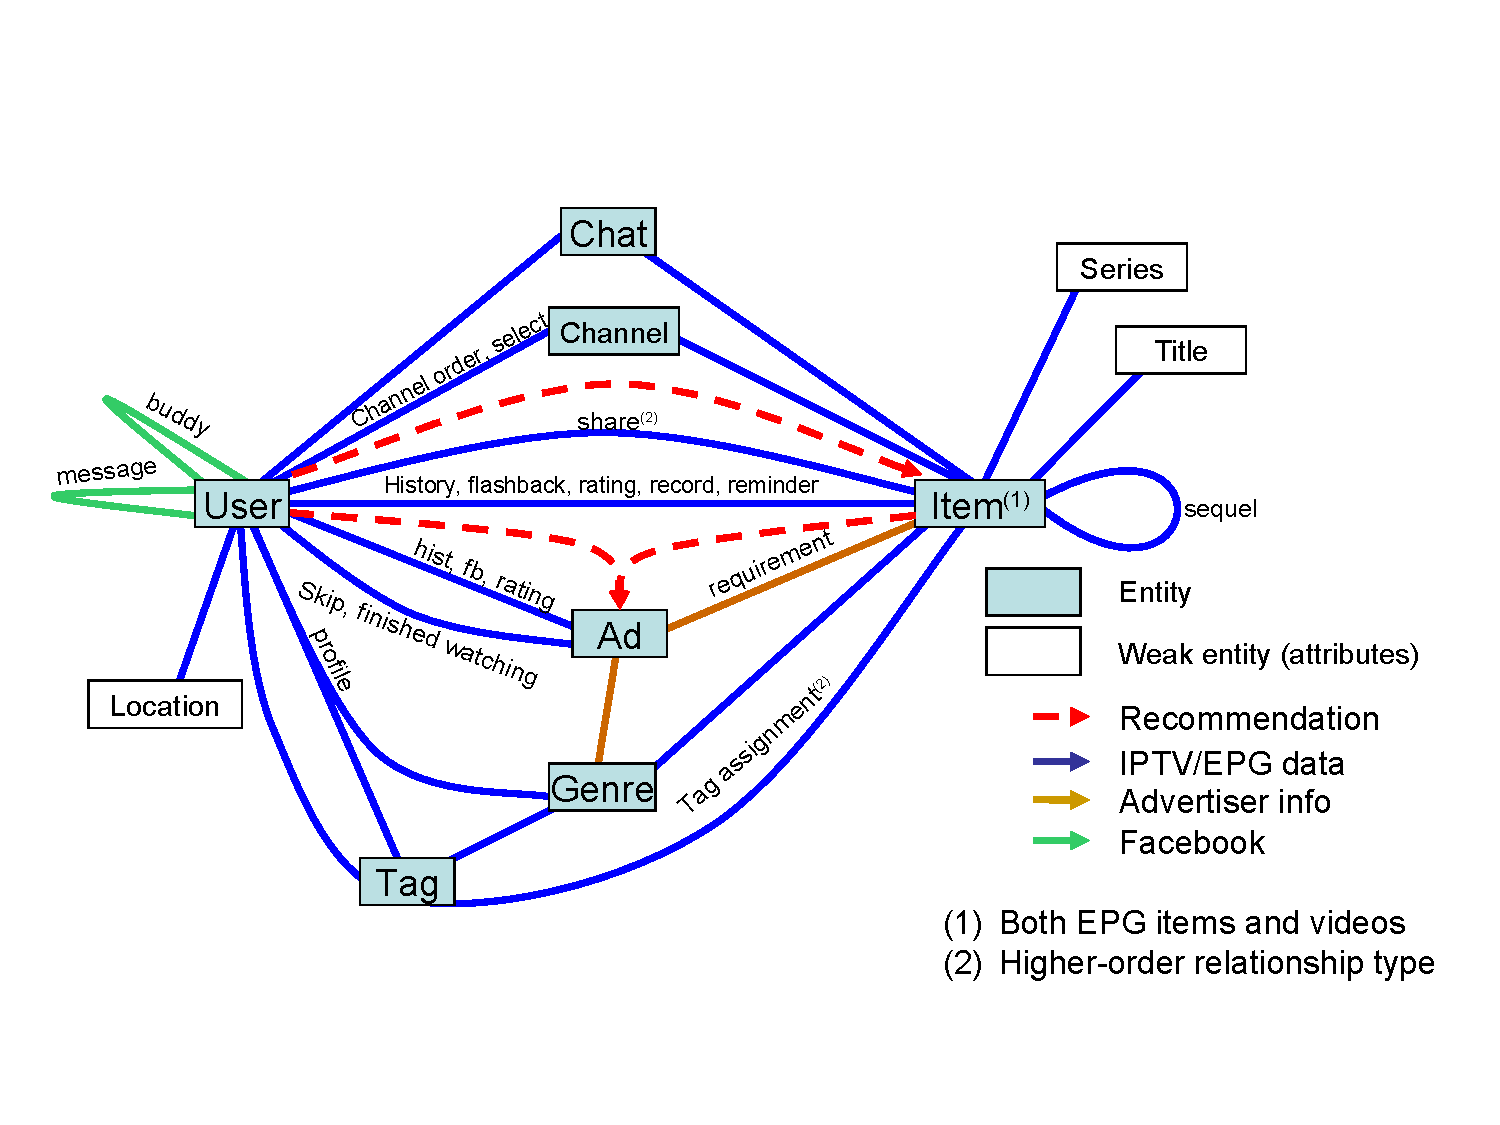
\includegraphics[width=.9\textwidth]{iptv-er}
  \caption{
    Entity-relationship diagram of the IPTV system.  Entities are
    represented by nodes and relationships by connections.
    Recommendation use cases are drawn as dashed red lines. 
    Any dataset usable by the Universal Recommender can be represented
    by such a graph. 
  }
  \label{fig:iptv-er}
\end{figure}

This example shows characteristics found in many recommender system
datasets:  The primary entity types are users and items, which are TV
programs in this case.  The main relationship types connect users and
items.  In our example these are view, flashback, rating, record and
reminder events.  This scenario shows a common feature of recommender systems:
several relationship connect the same entity types.  Other relationship
types connect secondary entities such as locations, genre, series and
titles.  User-user relationships are represented by message events and
buddy lists, both common in recommender systems.  This dataset also
contains higher-order relationship types, in form of tag assignments and
share events. 

This example also shows how difficult it is in general to find build a
good hybrid recommender system out of simple recommender system.  There
are so many relationship types that a hybrid recommender has too many
parameters to be optimized by trial and error. 

\section{Conclusion}
We proposed the Universal Recommender, a generic recommender system that
applies to any dataset consisting of entity and relationships of any
number of entity and relationship types.  
We showed how the Universal Recommender extends most known recommender
systems using Internet Protocol Televion as a case study.
We identified key machine learning and optimization problems that must be
studied to implement a successful Universal Recommender. 

As a real-world example illustrating use of the Universal Recommender,
we presented the Internet Protocol Televion (IPTV) recommender. 

\bibliographystyle{acm}
\bibliography{kunegis}

\end{document}

